\documentclass[a4paper,12pt,twoside]{article}
\usepackage[spanish]{babel}
\usepackage[utf8]{inputenc}
\usepackage{graphicx} %para insertar graficos/imagenes
\usepackage{amsmath} %para escribir matrices
\usepackage{amsfonts} %para poner \mathbb
\usepackage{float} %me deja usar la H de 'here' en los graficos para ponerlos donde yo quiera
\usepackage{anysize} %me permite definir los margenes como quiera
\usepackage{multirow} %para tablas con multicolumna
\usepackage{fancyhdr} % activamos el paquete
\usepackage{dcolumn}
\usepackage{multirow}

\usepackage{fixme}
\fxsetup{
    status=draft,
    author= carballeda ignacio,
    layout=inline, % also try footnote or pdfnote
}

\newcommand{\grad}{$^\circ$}

\newcommand{\codigoMateria}{66.10}
\newcommand{\nombreMateria}{Circuitos Electrónicos II}
\newcommand{\nroTP}{1}
\newcommand{\descripcionTP}{Informe Final}
\newcommand{\tituloTP}{Amplificador Clase G}
\newcommand{\facultad}{Facultad de Ingeniería}
\newcommand{\universidad}{Universidad de Buenos Aires}
\newcommand{\docentes}{Alberto Bertuccio\\Federico D'Angiolo}

\pagestyle{fancy} % seleccionamos un estilo
\fancyhead{}
\fancyfoot{}
\lhead{\nombreMateria \, (\codigoMateria)} % texto izquierda de la cabecera
\rhead{\facultad} % texto centro de la cabecera
\cfoot{\thepage}

\marginsize{2cm}{2cm}{1cm}{1.5cm} %izquierda, derecha, arriba, abajo

\newcommand{\Direcrotio}{./}
\newcommand{\HRule}{\rule{\linewidth}{1mm}}


% Símbolos de las unidades
% Se utiliza el comando \ensuremath{~} por seguridad
% Incluyo también gensymb que añade los comandos:
%\degree, \celsius, \perthousand, \micro and \ohm
%	º		ºC			o/oo		µ			Ω

\usepackage{gensymb}

% VOLT
\newcommand{\nV}{\ensuremath{~\mathrm{nV}}}
\newcommand{\uV}{\ensuremath{~\mu\mathrm{V}}}
\newcommand{\mV}{\ensuremath{~\mathrm{mV}}}
\newcommand{\volt}{\ensuremath{~\mathrm{V}}}

% HERTZ
\newcommand{\hz}{\ensuremath{~\mathrm{Hz}}}
\newcommand{\hertz}{\ensuremath{~\mathrm{Hz}}}
\newcommand{\Hz}{\ensuremath{~\mathrm{Hz}}}
\newcommand{\khz}{\ensuremath{~\mathrm{kHz}}}
\newcommand{\kHz}{\ensuremath{~\mathrm{kHz}}}
\newcommand{\Mhz}{\ensuremath{~\mathrm{MHz}}}
\newcommand{\MHz}{\ensuremath{~\mathrm{MHz}}}

% FARAD
\newcommand{\pF}{\ensuremath{~\mathrm{pF}}}
\newcommand{\nF}{\ensuremath{~\mathrm{nF}}}
\newcommand{\uF}{\ensuremath{~\mu\mathrm{F}}}
\newcommand{\mF}{\ensuremath{~\mathrm{mF}}}
\newcommand{\farad}{\ensuremath{~\mathrm{F}}}

% OHM
%\newcommand{\ohm}{\ensuremath{~\Omega}}
\newcommand{\nohm}{\ensuremath{~\mathrm{n}\ohm}}
\newcommand{\uohm}{\ensuremath{~\mu\ohm}}
\newcommand{\mohm}{\ensuremath{~\mathrm{m}\ohm}}
\newcommand{\kohm}{\ensuremath{~\mathrm{k}\ohm}}
\newcommand{\Mohm}{\ensuremath{~\mathrm{M}\ohm}}

% HENRY
\newcommand{\uHy}{\ensuremath{~\mu\mathrm{Hy}}}
\newcommand{\nHy}{\ensuremath{~\mathrm{nHy}}}
\newcommand{\mHy}{\ensuremath{~\mathrm{mHy}}}
\newcommand{\henry}{\ensuremath{~\mathrm{Hy}}}

% AMPERE
\newcommand{\fA}{\ensuremath{~\mathrm{fA}}}
\newcommand{\uA}{\ensuremath{~\mu\mathrm{A}}}
\newcommand{\nA}{\ensuremath{~\mathrm{nA}}}
\newcommand{\mA}{\ensuremath{~\mathrm{mA}}}
\newcommand{\amper}{\ensuremath{~\mathrm{A}}}

% SEGUNDOS
\newcommand{\nS}{\ensuremath{~\mathrm{ns}}}
\newcommand{\uS}{\ensuremath{~\mu\mathrm{s}}}
\newcommand{\mS}{\ensuremath{~\mathrm{ms}}}
\newcommand{\seg}{\ensuremath{~\mathrm{s}}}

% WATTS
\newcommand{\mW}{\ensuremath{~\mathrm{mW}}}
\newcommand{\watt}{\ensuremath{~\mathrm{W}}}

% DECIBELES
\newcommand{\dB}{\ensuremath{~\mathrm{dB}}}
\newcommand{\dBm}{\ensuremath{~\mathrm{dBm}}}

% señal
\newcommand{\vs}[1]{%
\ensuremath{~v_{\mathrm{#1}}}%
}
\newcommand{\is}[1]{%
\ensuremath{~i_{\mathrm{#1}}}%
}

% ctes
\newcommand{\VA}{\ensuremath{~\mathrm{V}_{\mathrm{A}}}}
\newcommand{\VT}{\ensuremath{~\mathrm{V}_{\mathrm{T}}}}
\newcommand{\Vth}{\ensuremath{~\mathrm{V}_{\mathrm{th}}}}
\newcommand{\VCC}{\ensuremath{~\mathrm{V}_{\mathrm{CC}}}}
\newcommand{\VBB}{\ensuremath{~\mathrm{V}_{\mathrm{BB}}}}
\newcommand{\VDD}{\ensuremath{~\mathrm{V}_{\mathrm{DD}}}}
\newcommand{\VGG}{\ensuremath{~\mathrm{V}_{\mathrm{GG}}}}
\newcommand{\VSS}{\ensuremath{~\mathrm{V}_{\mathrm{SS}}}}
\newcommand{\RB}{\ensuremath{~\mathrm{R}_{\mathrm{B}}}}
\newcommand{\RC}{\ensuremath{~\mathrm{R}_{\mathrm{C}}}}
\newcommand{\RE}{\ensuremath{~\mathrm{R}_{\mathrm{E}}}}
\newcommand{\RL}{\ensuremath{~\mathrm{R}_{\mathrm{L}}}}
\newcommand{\RG}{\ensuremath{~\mathrm{R}_{\mathrm{G}}}}
\newcommand{\RD}{\ensuremath{~\mathrm{R}_{\mathrm{D}}}}
\newcommand{\RS}{\ensuremath{~\mathrm{R}_{\mathrm{S}}}}
\newcommand{\Rs}{\ensuremath{~\mathrm{R}_{\mathrm{s}}}}
\newcommand{\R}[1]{%
\ensuremath{~\mathrm{R}_{\mathrm{#1}}}%
}
\newcommand{\I}[1]{%
\ensuremath{~\mathrm{I}_{\mathrm{#1}}}%
}
\newcommand{\V}[1]{%
\ensuremath{~\mathrm{V}_{\mathrm{#1}}}%
}
\newcommand{\Ip}[1]{%
\ensuremath{~\hat{\mathrm{I}}_{\mathrm{#1}}}%
}
\newcommand{\Vp}[1]{%
\ensuremath{~\hat{\mathrm{V}}_{\mathrm{#1}}}%
}
\newcommand{\ip}[1]{%
\ensuremath{~\hat{i}_{\mathrm{#1}}}%
}
\newcommand{\vp}[1]{%
\ensuremath{~\hat{v}_{\mathrm{#1}}}%
}
\newcommand{\A}[1]{%
\ensuremath{~\mathrm{A}_{\mathrm{#1}}}%
}
\newcommand{\nada}{\quad{}}


\newenvironment{items}{
\begin{itemize}
  \renewcommand{\labelitemi}{$\bullet$}
  \setlength{\itemsep}{3pt}
  \setlength{\parskip}{1pt}
  \setlength{\parsep}{1pt}
}{
\end{itemize}}



\begin{document}



\begin{titlepage}

\thispagestyle{empty}

\begin{center}


\includegraphics[scale=0.15]{fiuba}\\[0.1cm]
\textsc{\universidad}\\[0.2cm]
\large{\textsc{\facultad}}\\[0.2cm]

\end{center}

\vfill

\begin{center}
\underline{\Large{\nombreMateria\, (\codigoMateria)}}
\end{center}

\vfill
\begin{center}

\end{center}
\vfill

\begin{center}
\Huge{\textsc{ \tituloTP }}\\[.5cm]
	\begin{figure}[H]
		\centering
		%\includegraphics[width=.5\textwidth]{bessel}
	\end{figure}\HRule \\[0.1cm]
\Huge{\textbf{\descripcionTP}}\\[0.01cm]
\HRule\\[0.3cm]
\end{center}

\vfill



\begin{tabbing}
	FECHA: \today\\
\\
	INTEGRANTES:\hspace{-1cm}\=\+\hspace{1cm}\=\hspace{6cm}\=\\
		Gomez, Cristian	\>\>- \#89968\\
			\>\footnotesize{$<$crisgvenezia@gmail.com$>$}\\
		Pollitzer, Ivan Gustavo	\>\>- \#22922\\
			\>\footnotesize{$<$igpollitzer@gmail.com$>$}\\
		Carballeda, Ignacio	\>\>- \#91646\\
			\>\footnotesize{$<$carballeda.ignacio@gmail.com$>$}\\

\end{tabbing}

\begin{flushleft} \large
\emph{Docentes:}\\[.2cm]
\end{flushleft}
\begin{tabbing}
\docentes\\[.5cm]
\end{tabbing}

\vfill

\hrule
\vspace{0.2cm}

\noindent\small{\codigoMateria\, --- \nombreMateria \hfill \facultad}

\end{titlepage}


\newpage
\vfill
\tableofcontents
\vfill

\newpage
\section{Introducción}
\subsection{Amplificadores de Potencia}

Un amplificador debe satisfacer ciertos requerimientos especiales. Uno de los más importantes es el de entregar una señal con una cantidad específica de potencia a una carga con niveles aceptablemente bajos de distorsión. Otro objetivo común en el diseño es minimizar la impedancia de salida, de tal forma que la ganancia de tensión quede relativamente poco afectada por el valor de la impedancia de carga.

Los amplificadores de potencia  se clasifican generalmente en seis tipos: A, B, AB , C y G para diseños analógicos y clases D y E para los diseños de conmutación. 



\subsubsection*{Amplificadores Clase A}

Es la clase mas simplificada de un amplificador de potencia, en esta se usa un solo transistor. El emisor seguidor es la etapa de salida clase A mas utilizada. La corriente de salida circula durante todo el ciclo de la señal de entrada, ya que el transistor esta polarizado con una corriente continua. Esta es una de las grandes desventajas de este tipo de amplificador ya que consume potencia en ausencia de señal y por lo tanto es lógico esperar un rendimiento pobre que en general no supera el 25\%. Como ventaja la distorsión introducida suele ser baja. En la Figura~\ref{ampliA} se muestra un ejemplo de este tipo de amplificador.
 
\begin{figure}[H]
\centering
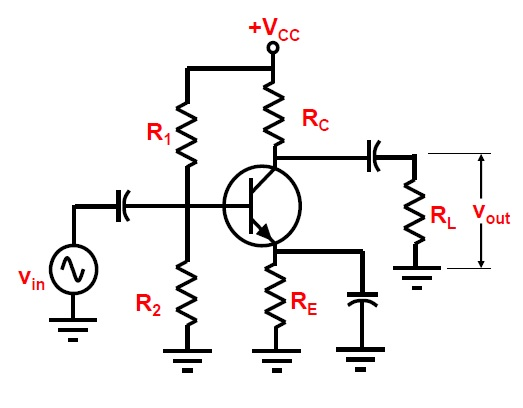
\includegraphics[scale=0.6]{img/Amplificador-clase-a.jpg}
\caption{Ejemplo, amplificador clase A}
\label{ampliA} 
\end{figure}

\medskip 
\subsubsection*{Amplificador Clase B}

Esta clase de amplificadores se compone de un par de transistores (uno PNP y otro NPN) conectados de forma tal que no se encuentren ambos en la zona de modo activo directo en el mismo instante de tiempo. Es decir, si suponemos tener una entrada senoidal, durante un semiciclo uno de los transistores se encuentra en la región activa, conduciendo corriente, mientras que el otro se encuentra en corte y durante el otro semiciclo viceversa.
 Una ventaja de esta amplificador sobre la clase A, es que los transistores no disipan potencia en ausencia de señal, lo cual mejora la vida útil de los transistores y el rendimiento notablemente, alcanzando un máximo del 78\%.
 La desventaja en este tipo de amplificadores es la llamada “distorsión por cruce”. Es fácil detectar su procedencia al analizar la Figura~\ref{ampliB}.

\begin{figure}[H]
\centering
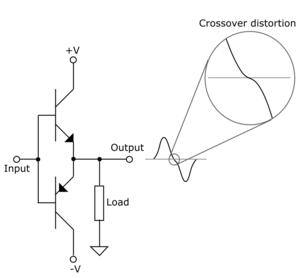
\includegraphics[scale=0.8]{img/ampliB.png}
\caption{Ejemplo, salida clase B.}
\label{ampliB} 
\end{figure}


Se observa que hay un intervalo de tensiones en el cual los transistores no conducen, ese rango generalmente esta dado por $\pm$0.7 V y esta dado por las curvas características de transferencia.

\medskip 
\subsubsection*{Amplificador Clase “AB”}


 Este tipo de amplificadores recurre a la misma topología utilizada en la etapa de salida de los amplificadores clase B, con la salvedad de que aquí en los transistores circulan una corriente de polarización a modo de reducir notablemente la “distorsión por cruce”.
 Existen diferentes formas de logra dicho tipo de polarización. Las mas sencillas implican agregar un resistor o diodos, por los que circula una corriente fija dada por el circuito de polarización o fuente de corriente. La otra forma es utilizar los circuitos conocidos como multiplicadores de VBE , que resulta ser la forma empleada en este trabajo práctico.


\medskip 
\subsubsection*{Amplificador Clase D}

Esta clase de amplificadores usa señales de pulso (digitales). El uso de técnicas digitales hace posible obtener una señal que varía a lo largo del ciclo completo para producir la salida a partir de muchas partes de la señal de entrada. La principal ventaja de la operación en clase D es que los transistores MOSFET de salida trabajan solo en corte y saturación por lo que teóricamente no se disipa potencia en forma de calor y la eficiencia general puede ser muy alta, de entre 90\% a 99\%. En la practica los MOSFETS solo disipan potencia cuando se encuentran conduciendo (saturación) debido a la pequeña resistencia de encendido que poseen, de todas maneras esta potencia es despreciable ya que la resistencia de encendido es del orden de las milésimas de ohm. Se utilizan transistores MOSFET ya que son los únicos capaces de conmutar a las elevadas frecuencias de trabajo, del orden de las centenas de KHz llegando a los MHz en algunos casos.

\newpage

\subsubsection*{Amplificadores Clase G}

Un amplificador clase G funciona conmutando fuentes de alimentación. Para analizar su funcionamiento tendremos en cuenta un circuito básico como se muestra en la Figura~\ref{ampliG}. Mientras el nivel de la señal de entrada sea pequeño (dentro del margen de +/- V1), el amplificador toma la potencia de la fuente V1. Si la señal de entrada excede el nivel de tensión dado por V1, el circuito automáticamente corta el suministro dado por V1 y conmuta a la fuente de alimentación V2 como puede verse en la Figura~\ref{ampliG_salida}. De esta forma la disipación de potencia es compartida por los transistores de salida, logrando así una menor disipación de potencia y una mayor eficiencia.
En la práctica, la clase G se considera linealmente pobre, comparada con la clase B, dado que la conmutación de las fuentes de alimentación se realiza mediante unos diodos, dando de esta manera un resultado alineal, ya que los mismos deben almacenar y desalojar cargas.
 
\begin{figure}[H]
 \centering
 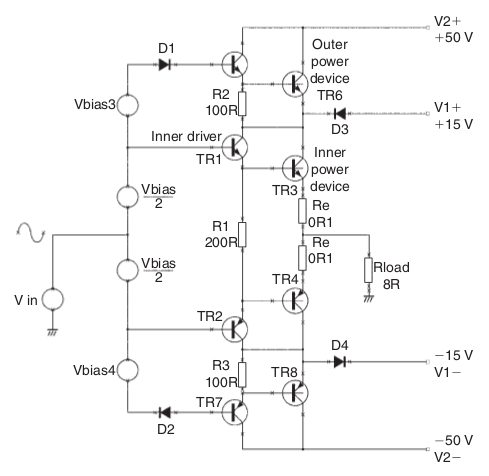
\includegraphics[scale=0.55]{img/ampliG.png}
 \caption{Ejemplo, amplificador clase G.}
 \label{ampliG} 
 \end{figure}
  
\begin{figure}[H]
 \centering
 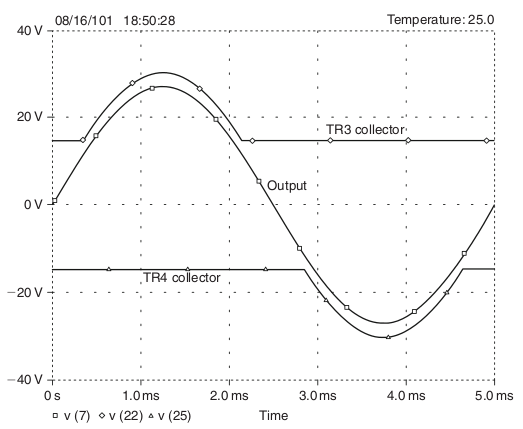
\includegraphics[scale=0.55]{img/ampliG_salida.png}
 \caption{Encendido de fuentes V2 en salidas clase G.}
 \label{ampliG_salida} 
 \end{figure}

\subsection{Inicio del desarrollo}

La arquitectura de los amplificadores esta compuesta generalmente de tres etapas principales. La primera etapa consta de una entrada diferencial, en la misma se realimenta negativamente la señal de salida; esta cuenta con un factor de ganancia pequeño. La segunda etapa es de amplificación de tensión (VAS); y por último la etapa de salida que corresponde a un buffer de corriente (ganancia de tensión unitaria).

La lectura del libro de Douglas-Self nos permitió aprender los conceptos básicos y la topología de un amplificador clase G. El siguiente diseño fue tomado directamente del libro y nuestro trabajo se basa en el mismo:

\begin{figure}[H]
	\centering
	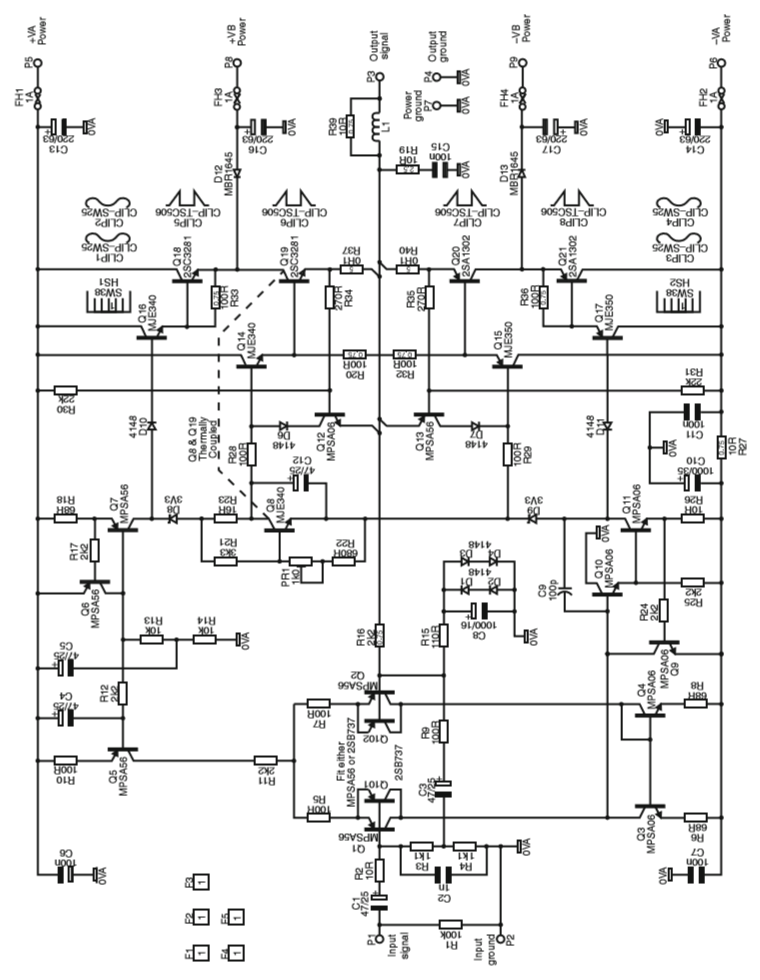
\includegraphics[scale=0.70]{img/ampli_douglas}
	\caption{Amplificador clase G , Douglas-Self}
	\label{douglas}
\end{figure}

\newpage
En el amplificador propuesto pudimos identificar las partes principales que componen el circuito. Como se observa en el siguiente diagrama en bloques.

\begin{figure}[H]
	\centering
	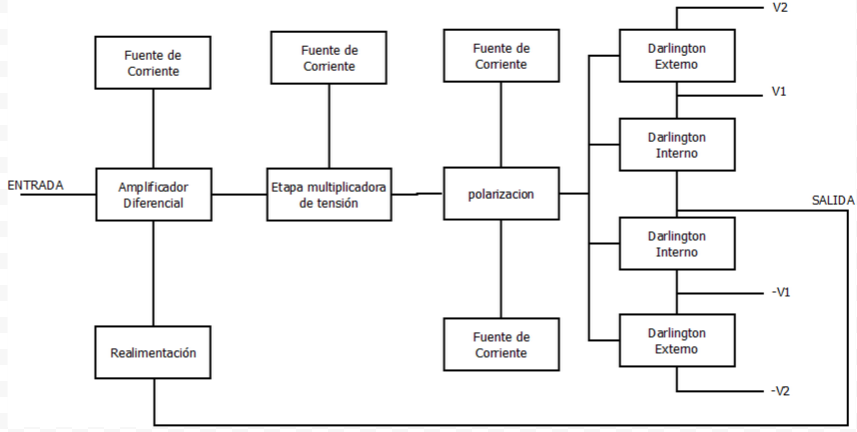
\includegraphics[scale=0.75]{img/ampli_bloques}
	\caption{Diagrama en bloques del amplificador clase G}
	\label{fig.1}
\end{figure}

Proponemos diseñar un circuito que incluya las partes que se pudieron identificar como así también cumpla las especificaciones que decidimos.


\newpage
\section{Objetivos}
\bigskip

Construir un un amplificador clase G que cumpla con las especificaciones planteadas. Dado que el circuito fue copiado de un libro, lo que se busca principalmente una compresión del mismo y, eventualmente, posibles mejoras.

\section{Especificaciones Propuestas} \label{sec:especificaciones}
\bigskip
Especificaciones iniciales de diseño:
\begin{itemize}
	\item Máxima Potencia de Salida:  $100\watt$ RMS @ $8\ohm$
	\item Clase: G
	\item THD: $<0.001 \%$ 
	\item Slew Rate: $>5V / \uS$
	\item Impedancia de entrada: $10\kohm$
	\item Sensibilidad: $1\volt$ RMS
	\item Alimentación: 
	\begin{itemize}
		\item Baja tensión: Apróx $ +/-20\volt$ 
		\item Alta tensión: Apróx $ +/-50\volt$
	\end{itemize}
\end{itemize}

\section{Motivación}
\bigskip

Un amplificador clase G está compuesto por dos o más niveles de alimentación que permiten incrementar la eficiencia del amplificador con respecto al clase B. Esto se logra ya que con tensiones bajas, se utilizará una fuente de tensión menor, preservando la máxima excursión posible sobre la carga que ofrece un clase B alimentado con la fuente de tensión mayor. Para señales con picos de baja amplitud en relación al valor medio, la mejora en la eficiencia es modesta. Sin embargo, en el caso en que la señal tenga picos considerables con respecto a su valor medio, la mejora es notable.

\newpage
\section{Desarrollo}
\subsection{Diseño Propuesto}
\begin{figure}[H]
	\centering
	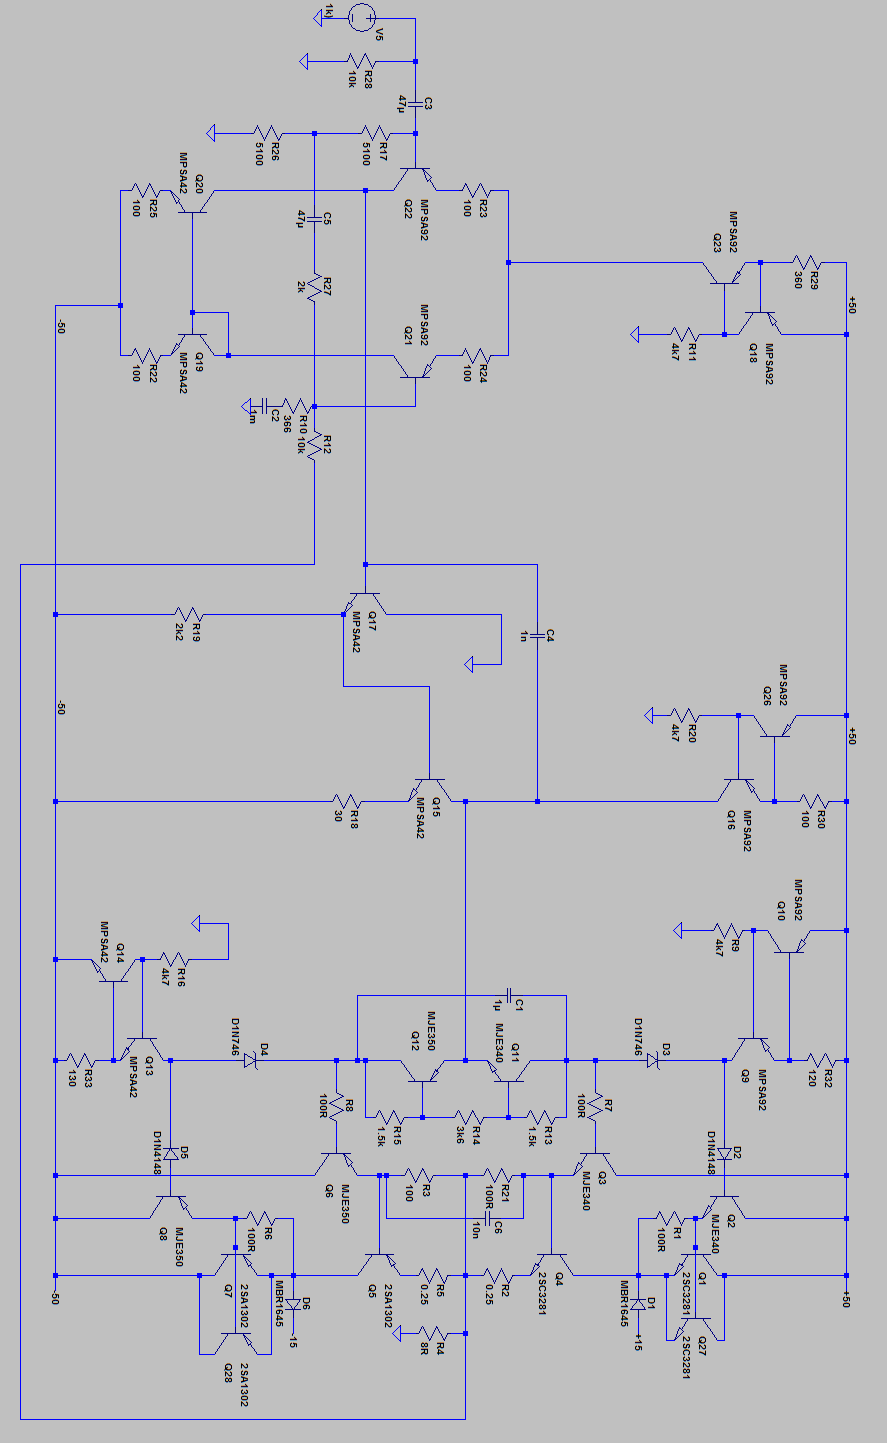
\includegraphics[scale=0.65]{img/circuito_propuesto}
	\caption{Diseño Propuesto}
	\label{diseniopropuesto}
\end{figure}
\subsection{Cambios al diseño original}

\subsubsection{Doble Multiplicador de $V_{be}$}
En lugar de un único multiplicador de Vbe, se usan dos para lograr así una mayor simetría. Esto tambien ayuda a disminuir el offset que se produce a la salida. En busqueda de mayor simetría en la etapa de salida nos tomamos la libertad de mover el VAS para ingresar la señal desde el centro. Como consecuencia a esto se debió agregar una fuente de corriente que polarice la etapa de salida inferior. Para evitar modificar la polarización, el VAS debe estar a cero potencial en el punto de conexión con la etapa de salida.

\subsubsection{Etapa de Potencia}
Esta etapa se modifico agregándole una fuente de corriente propia debido a que no toma la corriente de polarización de la etapa de salida como en el diseño original.

\subsubsection{Entrada Diferencial}
En el amplificador diferencial se reemplazó la carga resistiva por activa. También se utilizan dos transistores en paralelo en cada rama del par diferencial ya que esto permite disminuir los desapareamientos logrando que el beta equivalente sea mas estable. Ademas, de esta forma se disminuye a la mitad la corriente que circula por los mismos disminuyendo así el ruido shot en esta etapa.
 
\subsubsection{Fuentes de Corriente}
Se cambiaron los espejos de corriente por fuentes para que la misma sea invariante ante el ripple en las tensiones de alimentación. 

\subsubsection{Transistores de Salida en Paralelo}
Para reducir la corriente y temperatura en los transistores de potencia, se opto por conectarlos de a pares en paralelo.

\newpage
\section{Definiciones y Principales Especificaciones de un Amplificador}
\bigskip

En esta sección se presentan las definiciones de las características relevantes del amplificador que se desean optimizar.

\subsection{Distorsión Armónica Total (THD)}

La distorsión armónica, o THD,  es el cociente entre la suma de las potencias de las componentes armónicas con respecto a la potencia de la frecuencia fundamental que es la que excita al circuito, es decir,
\begin{equation} THD = \frac{\sum_{i=2}^{+\infty} P_i}{P_1} \end{equation}
donde $P_i$ es la potencia de la i-ésima armónica\footnote{Se tomó como convención que la primera armónica es la frecuencia fundamental.}. Sin embargo, en audio (y, por ende, la que adopta en presente trabajo) es más común la definición en términos de amplitudes de las armónicas,
\begin{equation} THD = \frac{\sqrt{\sum_{i_2}^{+\infty} V_i}}{V_1} \end{equation}

La THD es una medida de la alinealidad de un sistema producida principalmente por la transferencia alineal de las primeras dos estapas y el cruce o conmutación en la etapa de salida.

\subsection{Slew-Rate}

El Slew-Rate es la máxima velocidad de variación de tensión que puede reproducirse a la salida de un circuito electrónico, o bien,
\begin{equation} SR = \max \left(\left|\frac{dv_{out}(t)}{dt}\right|\right) \end{equation}

Cuando el sistema es excitado por una senoidal, para que la señal de salida no sufra este fenómeno, la frecuencia angular por la tensión pico debe ser menor al Slew-Rate del sistema. De esta manera, se obtiene un ancho de banda para gran señal dado por,
\begin{equation} f_{\max}= SR/(2 \pi V_p) \end{equation}
donde $f_{\max}$ es la frecuencia máxima sin deformación para una senoidal de amplitud $V_p$ a la salida del circuito y $SR$ es el Slew-Rate del circuito. Se debe a que la corriente disponible para cargar al capacitor de la etapa amplificadora de tensión es limitada.

\subsection{Relación Señal a Ruido (SNR)}

La relación señal a ruido\footnote{Se considerará ruido a toda señal no deseada en el circuito.} o SNR es una medida de la potencia de la señal util con respecto al nivel de ruido que produce el sistema y se expresa mediante,
\begin{equation} SNR=\frac{P_{S}}{P_{N}} \end{equation}

Es deseable obtener una SNR elevada.

\subsection{Fuentes de Ruido Intrínsecas}

En esta subsección se analizan los distintos tipos de ruidos presentes en el amplificador.

\subsubsection{Ruido Térmico o Ruido Johnson}

Es producido por los movimientos aleatorios de los electrones en componentes que disipan energía (resistores, transistores).

\subsubsection{Ruido Shot}

Es el ruido asociado a la circulación de corriente a través de una barrera de potencial y es proporcional a la corriente en continua que circula. Por lo tanto, para reducir este tipo de ruido es necesario mantener la corriente DC lo más pequeña posible.

\subsubsection{Ruido Popcorn}

Asociado a deficiencias en el proceso de fabricación de semiconductores. En el diseño no se tiene control sobre este tipo de ruido.

\subsection{Offset}

La presencia de desapareamientos en los componentes, en especial en los transitores del par diferencial de entrada, y los corrimientos con la temperatura, pueden producir tensiones a la salida incluso en la ausencia de una señal de entrada. Esto es importante ya que limita la resolución del amplificador. Es posible representar el efecto de todos estos desapareamientos a los efectos de la entrada del amplificador mediante dos cantidades: la tensión de offset y la corriente de offset. Resulta importante escoger los transistores del par diferencial con características muy similares, es decir, con valores de $\beta$ y $V_{BE}$ aproximadamente iguales.

\subsection{Eficiencia}

La eficiencia de un amplificador se define como el cociente entre la potencia media entregada a la carga y la potencia media que entregan las fuentes de alimentación, es decir,
\begin{equation} \eta = \frac{P_{CARGA}}{P_{FUENTES}} \end{equation}

\subsection{Respuesta en Frecuencia y Ancho de Banda}

La ganancia en función de la frecuencia de la señal que excita al sistema se denomina respuesta en frecuencia del circuito. Idealmente, el amplificador de audio debería presentar una ganancia constante para el rango de frecuencias del espectro audible, es decir, entre los $20\Hz$ y los $20\kHz$. La frecuencia para la cual la ganancia cae $3$ dB con respecto al valor en la banda mencionada, determina el ancho de banda del amplificador.

\subsection{Sensibilidad}

Es la máxima amplitud de la tensión de entrada para la cual la salida amplificada no recorta.

\subsection{Impedancia de Entrada y Salida}

\subsubsection*{Impedancia de Entrada}


 Es la impedancia equivalente que vería un generador aplicado a la entrada del amplificador. Para el caso particular de este tipo de amplificador (de tensión) buscamos que sea relativamente alta y no cargue a la etapa anterior. Claramente depende de la frecuencia de operación pero un valor típico para el rango de audiofrecuencias es de 10K $\ohm$.
\medskip 
\subsubsection*{Impedancia de Salida}


Es la impedancia equivalente que vería un generador aplicado a la salida del amplificador. En el caso particular del amplificador de audio buscamos que sea muy baja dado que las cargas son relativamente bajas y de lo contrario nos acortarían la amplitud de la señal de salida. Claramente depende de la frecuencia de operación pero un valor típico para el rango de audiofrecuencias es de décimas o centésimas de $\ohm$.


\newpage
\section{Simulaciones}
\subsection{Polarización}
\begin{figure}[H]
	\centering
	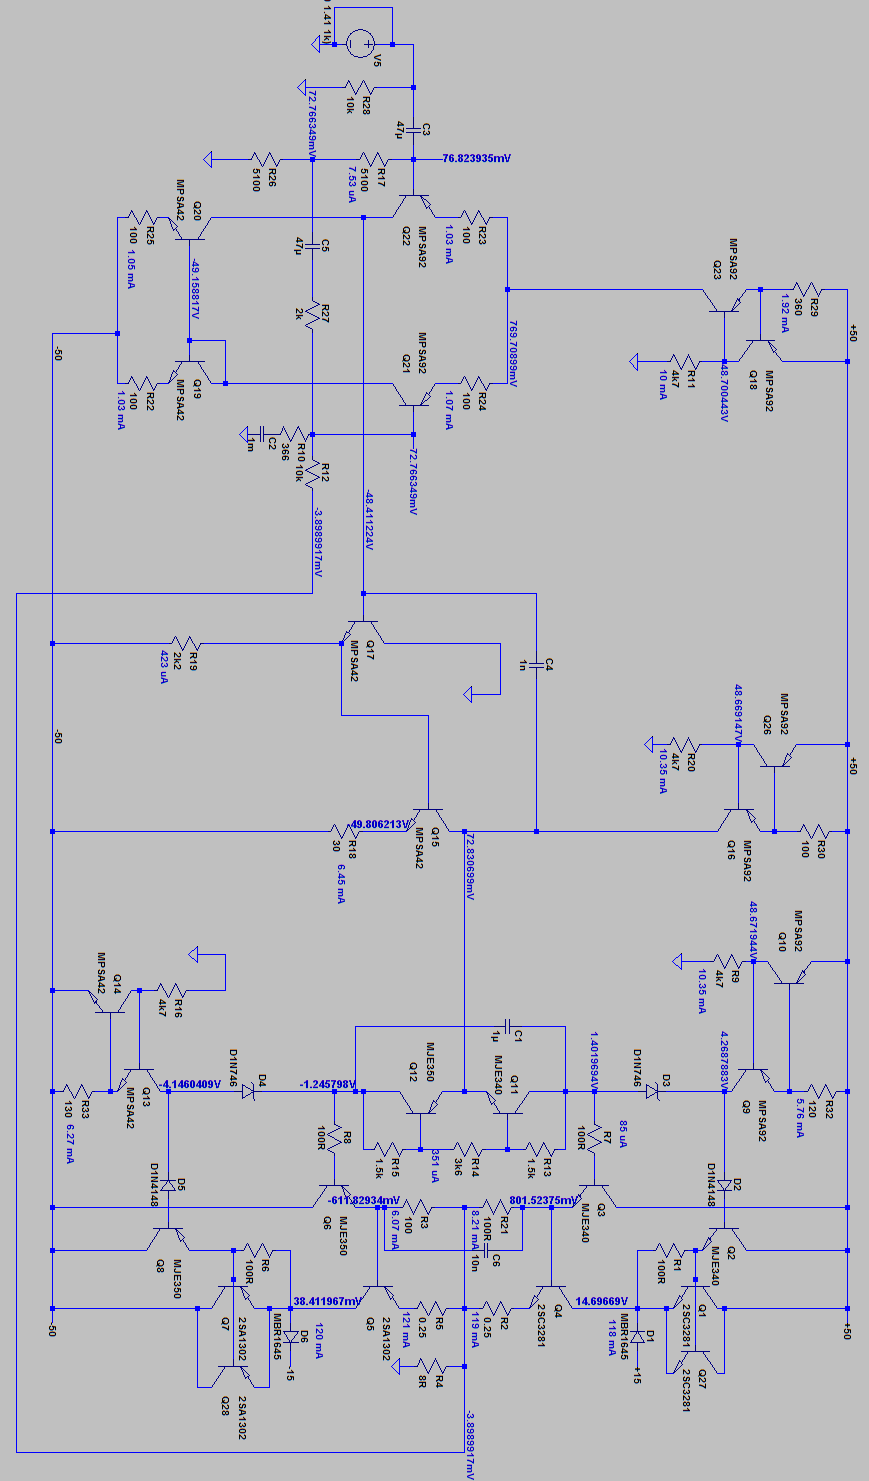
\includegraphics[scale=0.65]{img/polarizacion}
	\caption{Polarización}
	\label{fa}
\end{figure}


\subsection{Ganancia}
\subsubsection{Ganancia Lazo Abierto}
$A_{ol}=xx\dB$ 

\subsubsection{Ganancia Lazo Cerrado}
$A_{cl}=29.37\dB$ 

\subsection{Respuesta en Frecuencia}
Ancho de banda (caída $3 \dB$ ) es de 33 $\kHz$

\begin{figure}[H]
\centering
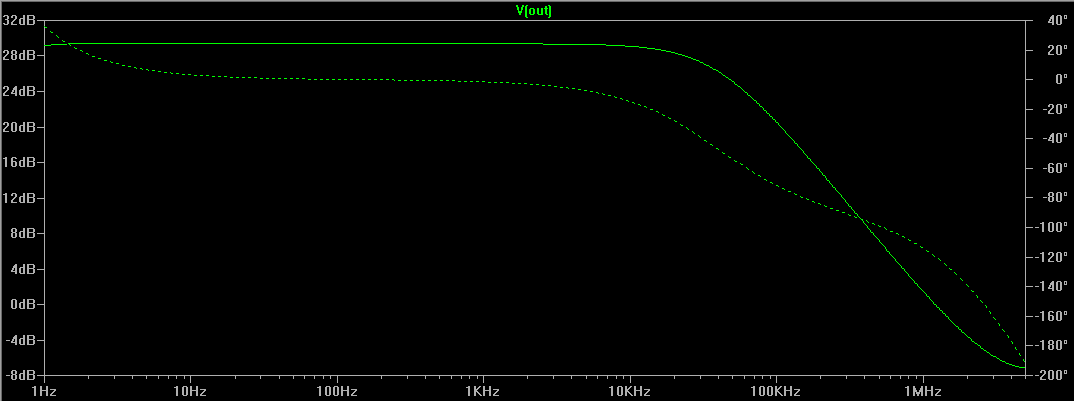
\includegraphics[scale=0.6]{img/ancho_de_banda}
\caption{Ancho de Banda}
\label{ancho_banda} 
\end{figure}

\subsection{Impedancia de Entrada}
Se estimo dividiendo la tensión del generador por su corriente. El resultado a $1 \kHz$ fue de aproximadamente $7 \kohm$.
\subsection{Impedancia de Salida}
Se pasivo el generador de señal y se coloco una fuente en la salida desacoplada por un capacitor. Realizando el mismo procedimiento que en el punto anterior, se estima una impedancia de salida de aproximadamente  $480 \mohm$ (a una frecuencia de $1 \khz$)

\subsection{Estabilidad}
Cuando la ganancia es de  $0\dB$ la fase es de $-118\degree$, esto sucede a $1.21$ $\MHz$.
El margen de fase (MF), es entonces de $62\degree$ , teniendo de esta forma un sistema estable.

\begin{figure}[H]
\centering
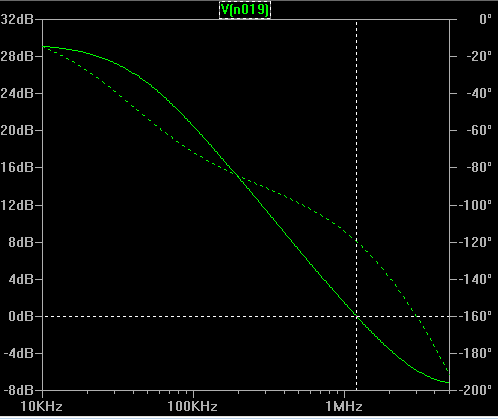
\includegraphics[scale=0.6]{img/estabilidad}
\caption{Estabilidad}
\label{estabilidad} 
\end{figure}


\subsection{Sensibilidad}

Para lograr $40 \volt$ a la salida se necesitaron $1.35 \volt$ en la entrada.

\begin{figure}[H]
\centering
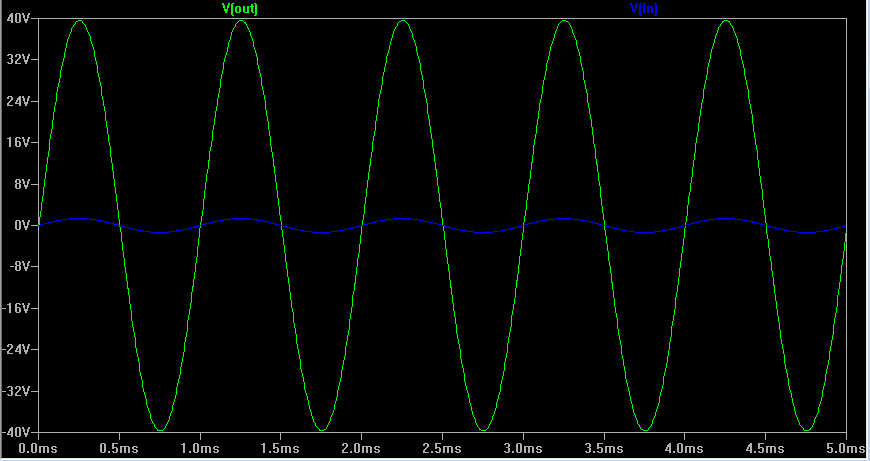
\includegraphics[scale=0.6]{img/sensibilidad}
\caption{sensibilidad}
\label{sens} 
\end{figure}


\subsection{Slew-Rate}

Para simular el slew-rate se puso una señal cuadrada en la entrada del amplificador, luego, se tomaron dos puntos en la salida con los cuales se calculo la pendiente.
Se obtuvo un slew-rate de $1.82 \frac{\volt}{\uS}$

\begin{figure}[H]
\centering
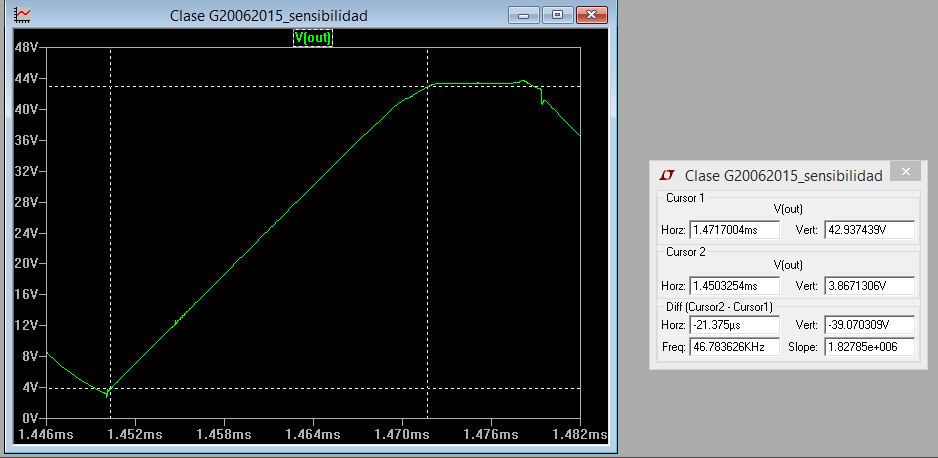
\includegraphics[scale=0.6]{img/slew_rate}
\caption{Slew-Rate}
\label{slew} 
\end{figure}



\subsection{Distorsión}

El THD a lazo cerrado frecuencia $1 \kHz$ y $1.35 \volt$ pico resultó ser de  THD=$0.002\%$.
Con la misma entrada y a una frecuencia de $10 \kHz$ THD=$0.005\%$


\begin{figure}[H]
\centering
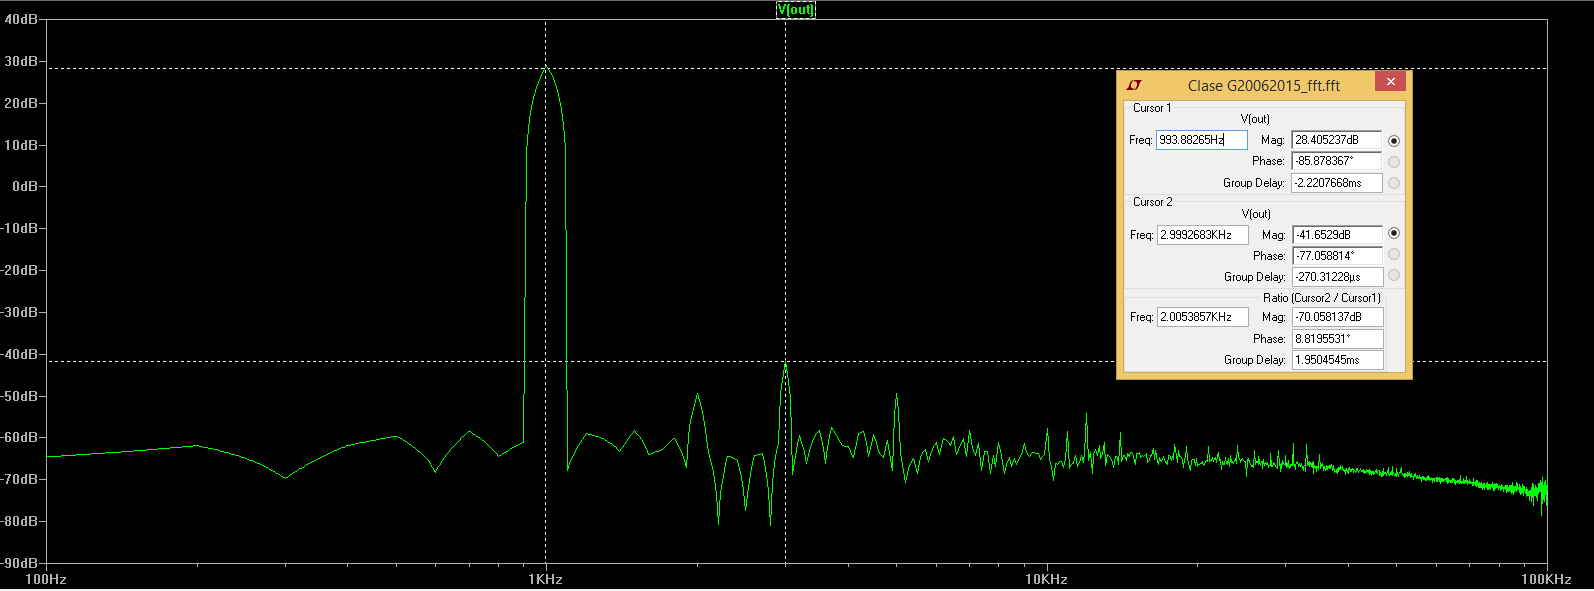
\includegraphics[scale=0.5]{img/fft}
\caption{fft}
\label{fft} 
\end{figure}



\newpage
\section{Realización del Circuito}
\subsection{Criterios de Diseño en PCB}
\subsection{Disipación de Calor}
\subsection{Circuito Impreso }
\subsection{Fotos}

\newpage
\section{Mediciones}
\subsection{Polarización}
\subsection{Ganancia}
\subsection{Respuesta en Frecuencia}
\subsection{Impedancia de Entrada}
\subsection{Impedancia de Salida}
\subsection{Slew Rate}
\subsection{THD}

\newpage

\section{Conclusiones}

\section{Software utilizado}
\begin{itemize}
\item KiCad - Diseño PCB
\item LTSpice - Simulación
\item \LaTeX - Confección del informe
\item Github - Control de versiones
\end{itemize}
\section{Bibliografía}

\begin{itemize}
\item Designing Audio Power Amplifiers - Bob Cordell
\item Audio Power Amplifier Design Handbook - Douglas Self 

\end{itemize}
\end{document}